\documentclass{sa}
\usepackage{array} %dla poziomego wyrownania (m) w tabeli
\usepackage{soul}

\newcommand{\ang}[1]{(ang. \emph{#1})}
\renewcommand{\vec}[1]{\ensuremath\mathbf{#1}}
\newcommand{\grad}{\ensuremath\nabla}
\let\avg\overline

\usetikzlibrary{datavisualization}
\usetikzlibrary{datavisualization.formats.functions}

\usepackage{hyperref}
\graphicspath{{03_regularyzacja/}}
\subtitle{Regularyzacja}
\begin{document}
\begin{frame}
\titlepage
\end{frame}

\begin{frame}{Schodzenie po gradiencie \ang{gradient descent}}
\centering
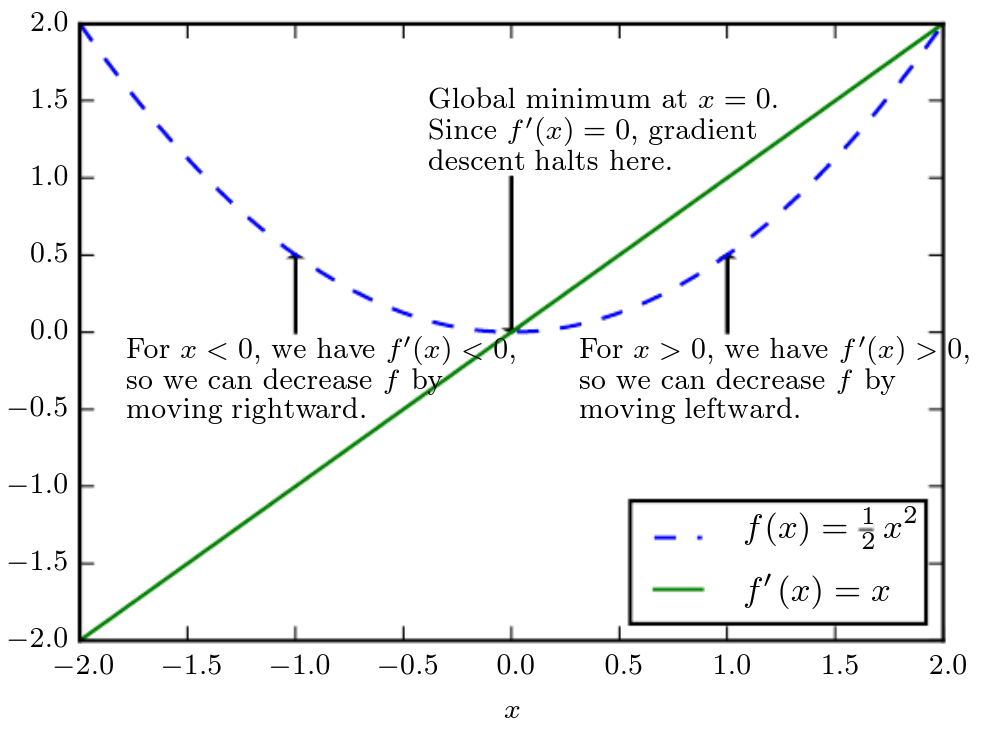
\includegraphics[width=.87\textwidth]{grad.png}
{\vfill\footnotesize I. Goodfellow, Y. Bengio, A. Courville \emph{Deep Learning} MIT Press 2016, str. 80}
\end{frame}

\begin{frame}{Schodzenie po gradiencie \ang{gradient descent}}
\centering
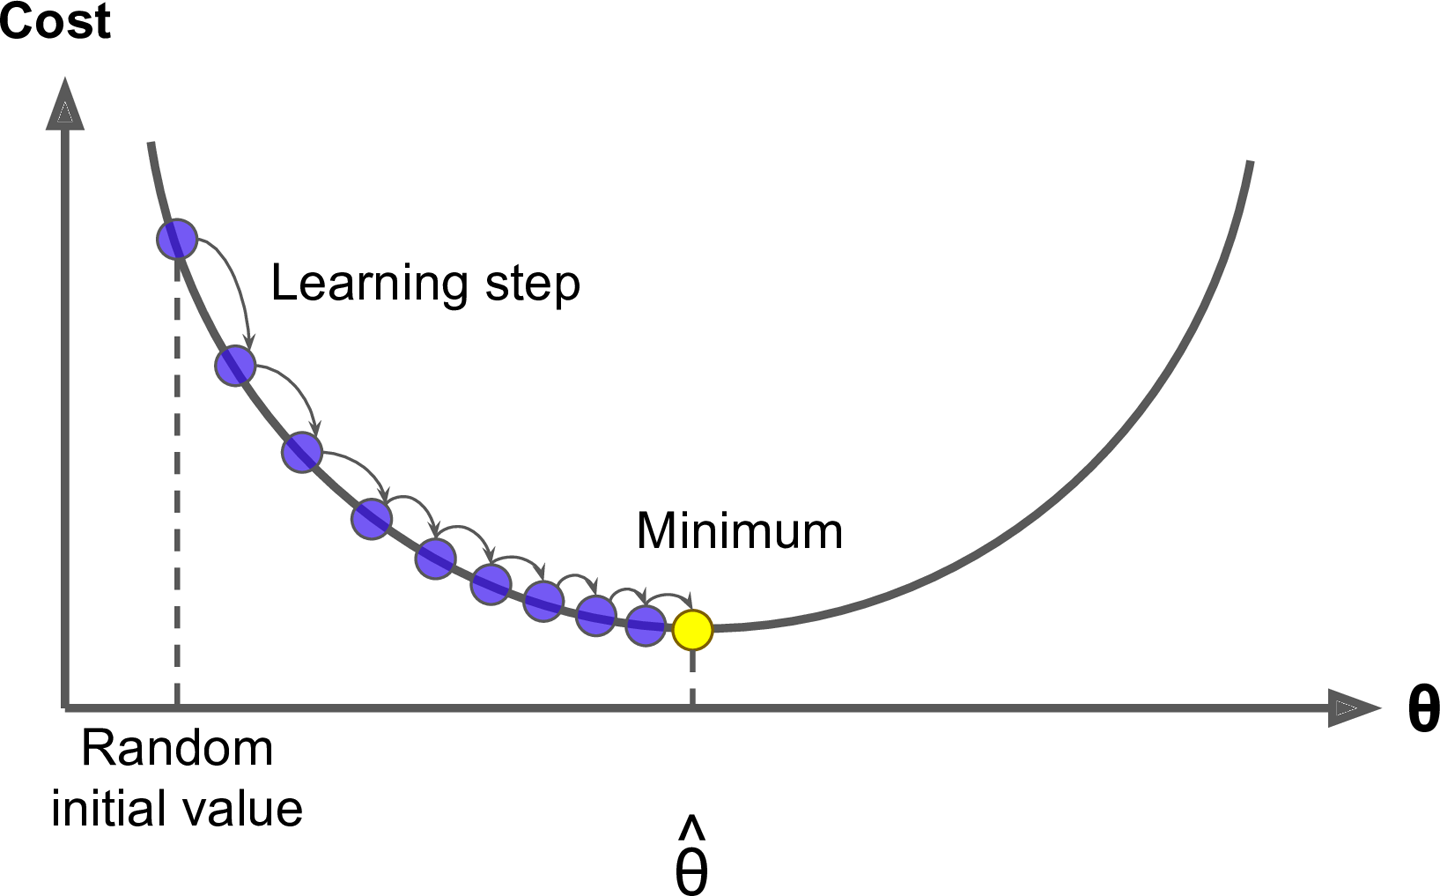
\includegraphics[width=.95\textwidth]{grad2.png}
{\vfill\footnotesize A. Géron, \emph{Hands-On Machine Learning with Scikit-Learn and TensorFlow} 2017, str. 111}
\end{frame}

\begin{frame}{Schodzenie po gradiencie \ang{gradient descent}}
\[ J(w, b) = \frac{1}{n}\sum_{i=1}^n \left(wx_i+b-y_i\right)^2 \]
\[ \grad J(w,b) = \begin{bmatrix}
\frac{1}{n}\sum_{i=1}^n 2x_i\left(wx_i+b-y_i\right) \\
\frac{1}{n}\sum_{i=1}^n 2\left(wx_i+b-y_i\right)
\end{bmatrix}
=
\frac{2}{n}\sum_{i=1}^n 
\left(wx_i+b-y_i\right) \begin{bmatrix}
x_i \\
1
\end{bmatrix}
\]
\[
\begin{bmatrix}
w' \\ b'
\end{bmatrix}
=
\begin{bmatrix}
w \\ b
\end{bmatrix}
-\varepsilon \grad J(w,b)
\]
\end{frame}

\begin{frame}{Prosiaki schodzące po gradiencie}
\begin{center}
\begin{tabular}{rrrrrr}
krok & $w$ & $b$ & $MSE$ & $\grad_w MSE$ & $\grad_b MSE$ \\
\hline
0 & 0 & 0 & $1280750$ & $-27700$ & $-1035$ \\
1 & $166.20$ & $6.21$ & $840233$ & $22433$ & $805$ \\
2 & $31.60$ & $1.38$ & $551427$ & $-18159$ & $-684$ \\
3 & $140.56$ & $5.48$ & $362082$ & $14708$ & $522$ \\
\ldots \\
$3102$ & $85.01$ & $49.96$ & $0.001$ & $0.002$ & $-0.014$ \\
\ldots \\
$6590$ & $85.00$ & $50.00$ & $0.000$ & $0.000$ & $0.000$ \\
\end{tabular}
\end{center}
\end{frame}


\begin{frame}{Prosiaki schodzące po gradiencie}
\begin{center}
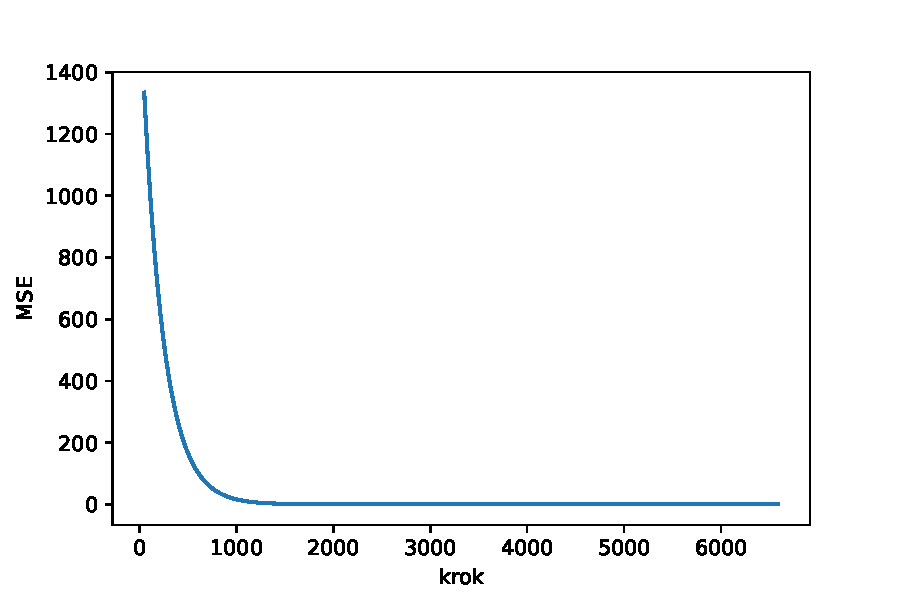
\includegraphics[width=.9\textwidth]{grad-prosiaki.pdf}
\end{center}

Warunek stopu: $MSE<1^{-10}$ lub $\grad J<1^{-10}$
\end{frame}

\begin{frame}{Stochastyczne schodzenie po gradiencie}
\begin{block}{\emph{Stochastic gradient descent}}
Jeżeli przykładów jest dużo, to schodzenie po gradiencie może być powolne.
Zamiast tego w każdym kroku wybieramy losowo \alert{jeden} przykład uczący i obliczamy gradient wyłącznie na jego podstawie.
\end{block}
\end{frame}

\begin{frame}{Stochastyczne schodzenie po gradiencie}
\centering
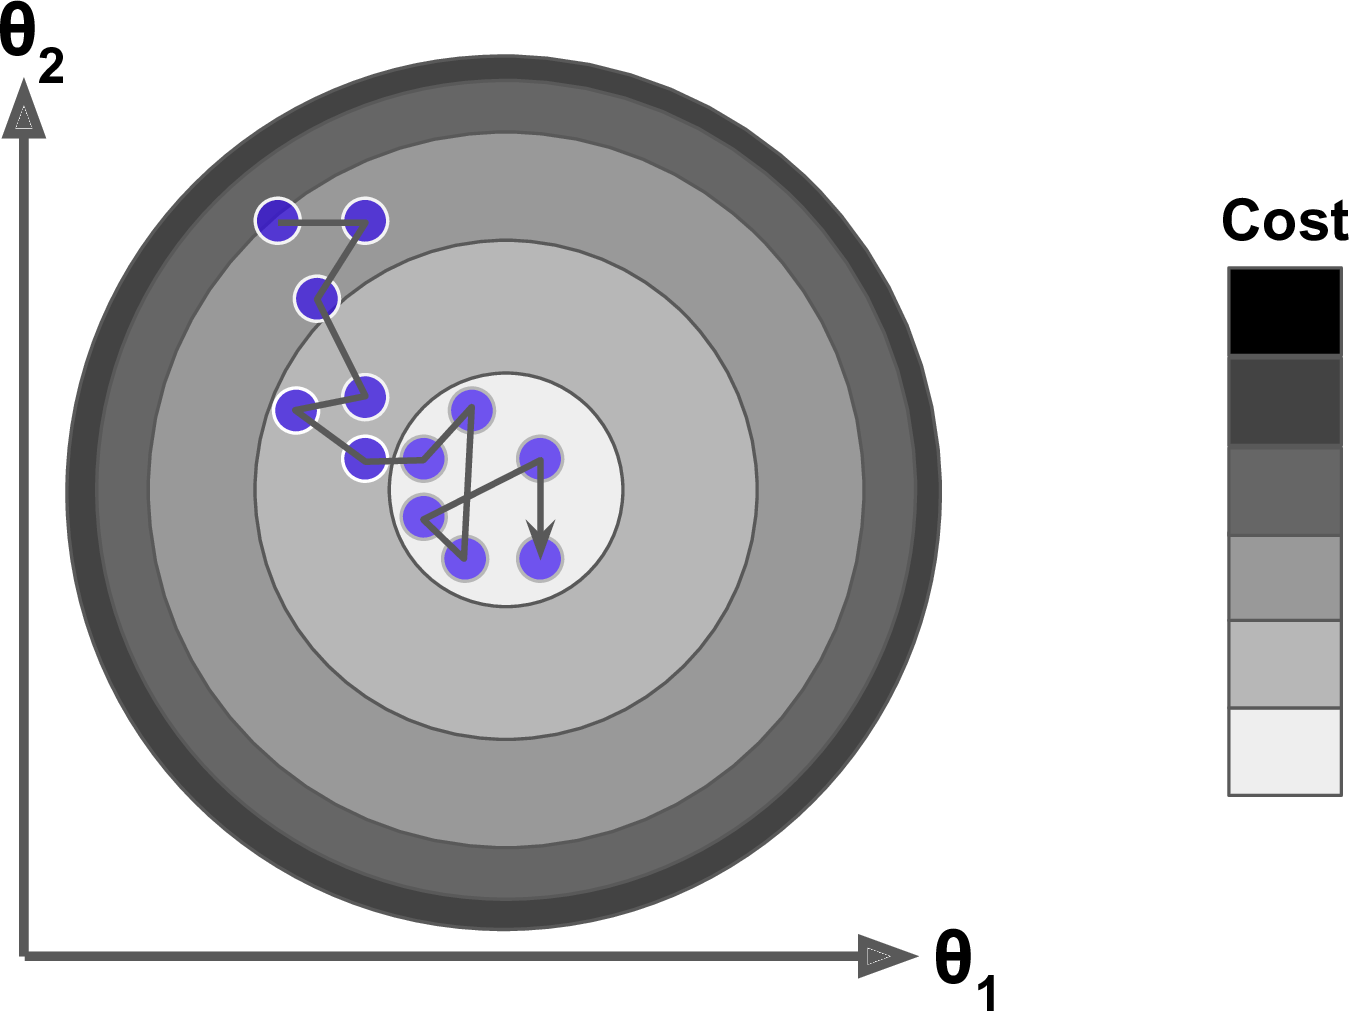
\includegraphics[width=.7\textwidth]{sgd.png}
{\vfill\footnotesize A. Géron, \emph{Hands-On Machine Learning with Scikit-Learn and TensorFlow} 2017, str. 117}
\end{frame}

\begin{frame}{Prosiaki stochastycznie schodzące po gradiencie}
\begin{center}
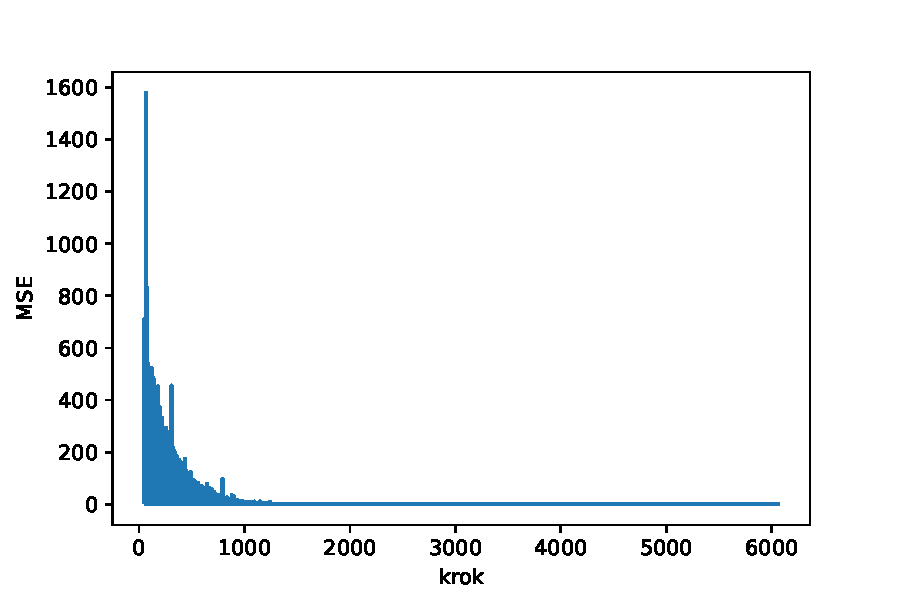
\includegraphics[width=.9\textwidth]{sgd-prosiaki.pdf}
\end{center}

Warunek stopu: $MSE$ przez ostatnie 10 kroków $<1^{-10}$
\end{frame}

\begin{frame}{Schodzenie po gradiencie z mini-grupami}
\begin{block}{\emph{Mini-batch gradient descent}}
W kolejnych krokach schodzenia po gradiencie wybieramy (niewielki) podzbiór przykładów uczących do obliczeń
\end{block}
\begin{itemize}
\item stabilniejszy
\item zysk wydajnościowy z obliczeń macierzowych
\end{itemize}
\end{frame}


\begin{frame}{Problemy ze schodzeniem po gradiencie}
\centering
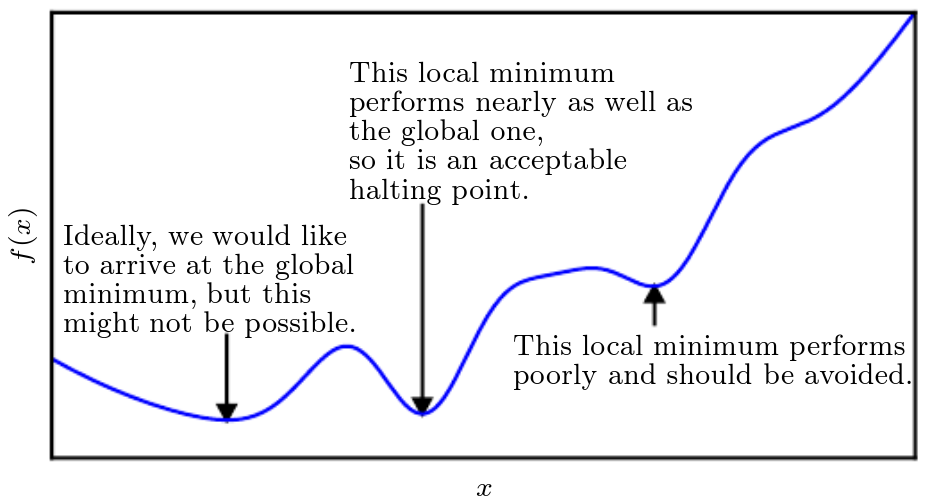
\includegraphics[width=\textwidth]{grad-problemy.png}
{\vfill\footnotesize I. Goodfellow, Y. Bengio, A. Courville \emph{Deep Learning} MIT Press 2016, str. 81}
\end{frame}

\begin{frame}{Problemy ze schodzeniem po gradiencie}
\centering
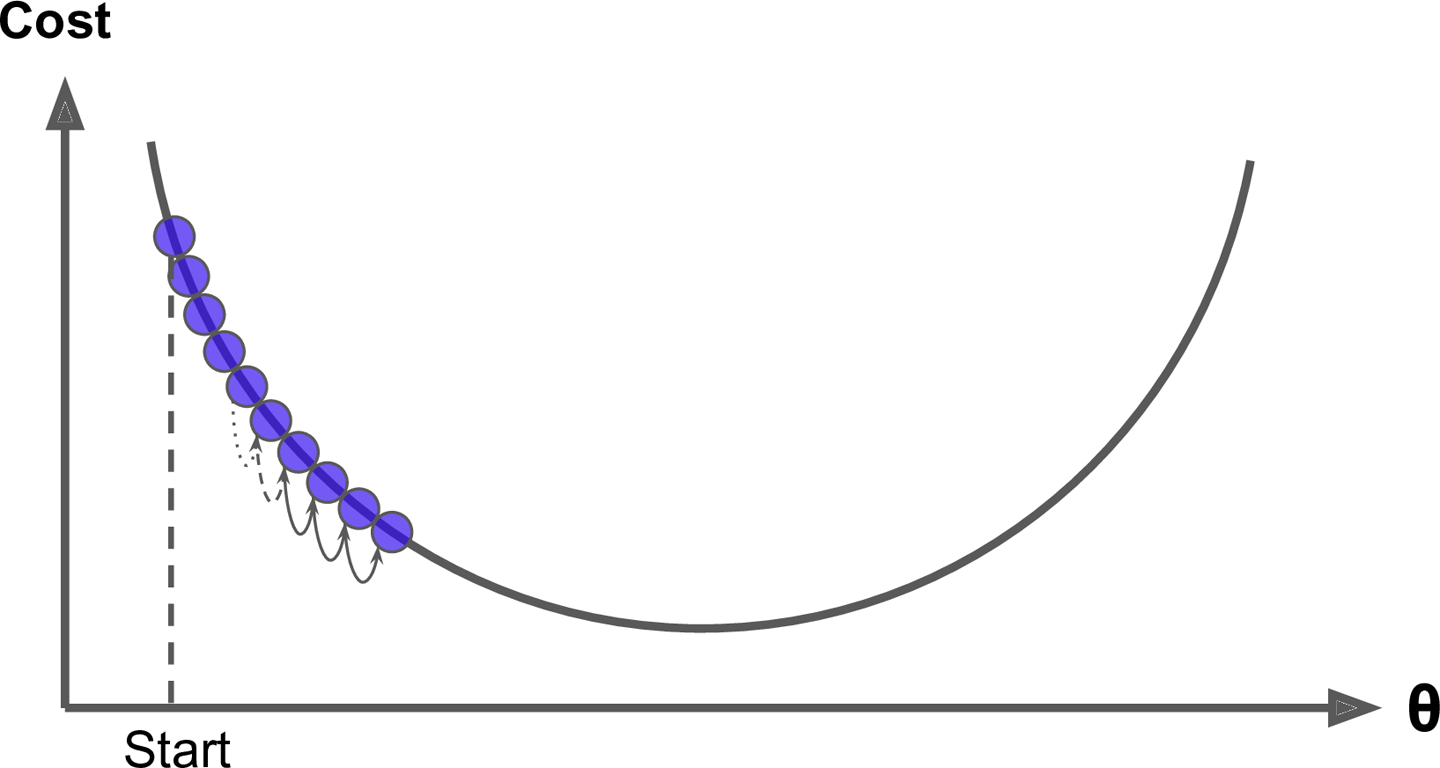
\includegraphics[width=.95\textwidth]{grad-e-toosmall.png}
{\vfill\footnotesize A. Géron, \emph{Hands-On Machine Learning with Scikit-Learn and TensorFlow} 2017, str. 112}
\end{frame}

\begin{frame}{Problemy ze schodzeniem po gradiencie}
\centering
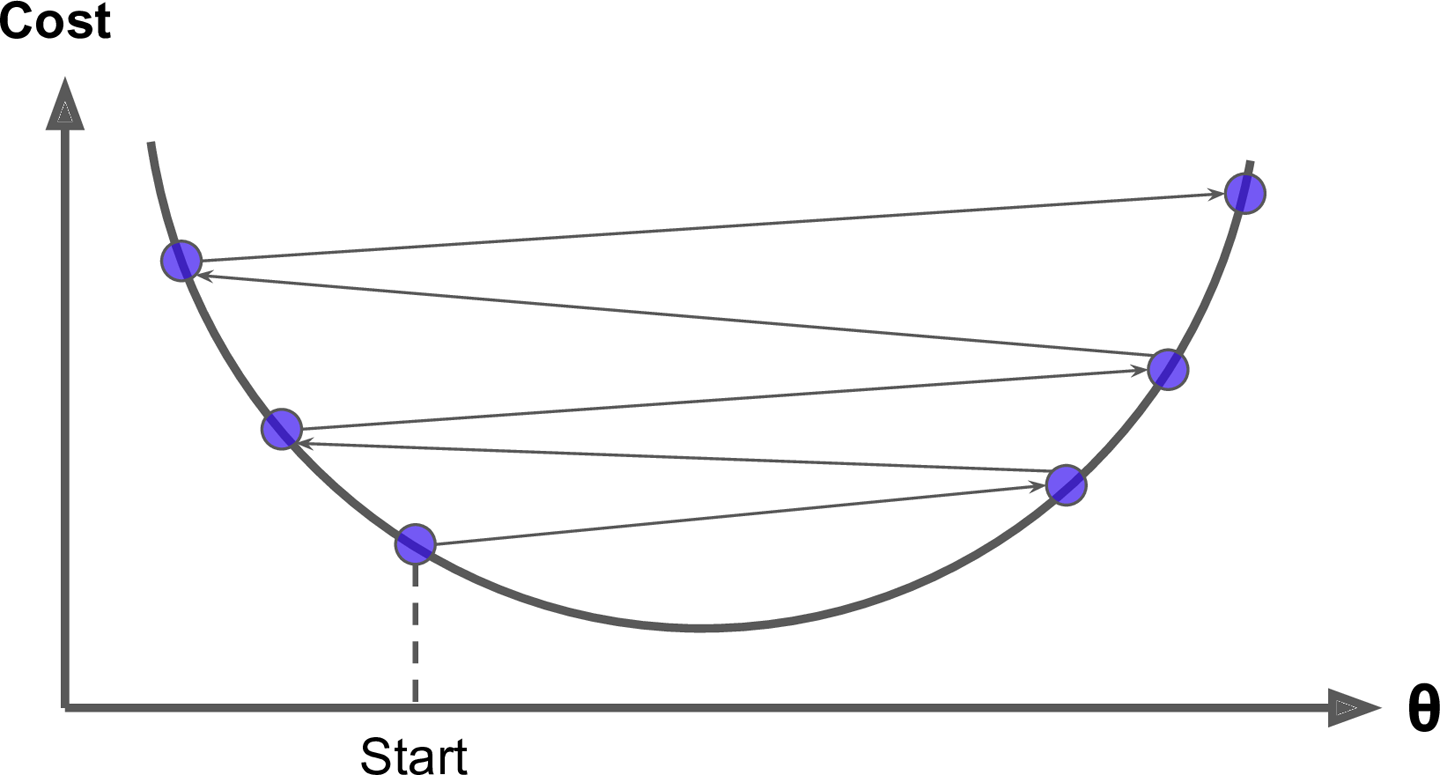
\includegraphics[width=.95\textwidth]{grad-e-toolarge.png}
{\vfill\footnotesize A. Géron, \emph{Hands-On Machine Learning with Scikit-Learn and TensorFlow} 2017, str. 112}
\end{frame}

\begin{frame}{Problemy ze schodzeniem po gradiencie}
\centering
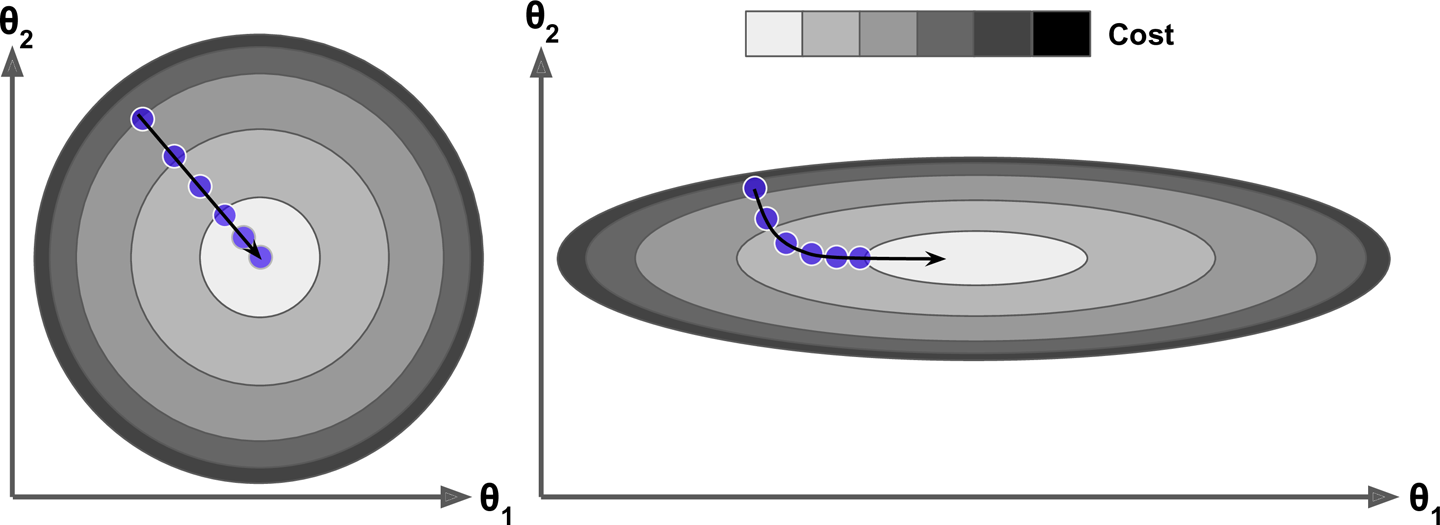
\includegraphics[width=.95\textwidth]{grad-nofscaling.png}
{\vfill\footnotesize A. Géron, \emph{Hands-On Machine Learning with Scikit-Learn and TensorFlow} 2017, str. 113}
\end{frame}

\begin{frame}{Skalowanie}
\begin{description}
\item[standaryzacja] \[ X_{i,j} = \frac{X_{i,j}-\overline{X_{\cdot,j}}}{\sigma_{X_{\cdot,j}}} \]
\item[min-max] \[ X_{i,j} = \frac{X_{i,j}-\min_k\{X_{k,j}\}}{\max_k\{X_{k,j}\}-\min_k\{X_{k,j}\}} \]
\end{description}

\vfill
\alert{Czym różnią się te dwa podejścia?}
\end{frame}

\begin{frame}{Trochę bardziej skomplikowany problem regresji}
\[ y=0{,}02x^3+10x+5+N(0,100) \]
niebieski: proces, pomarańczowy: zb. treningowy, zielony: zb. walidujący
\centering
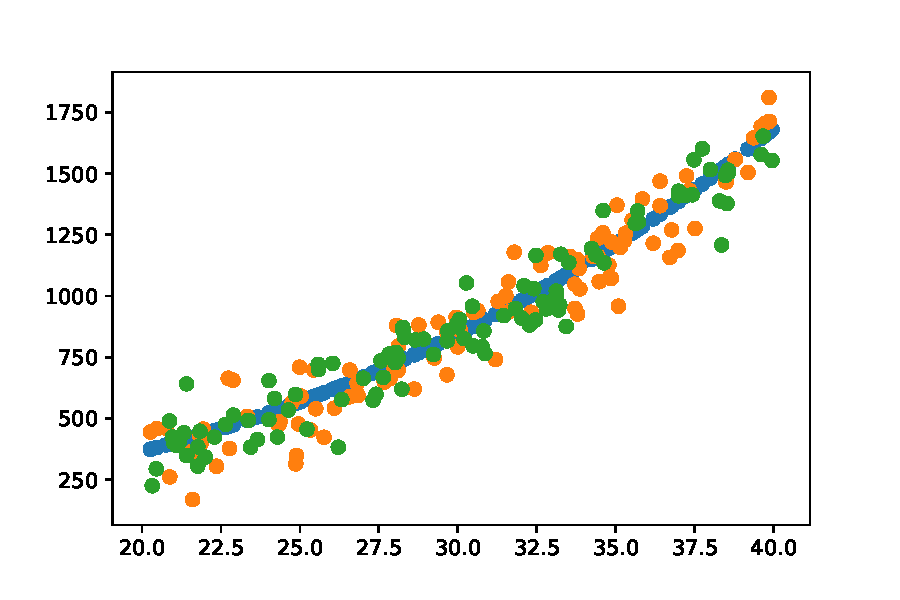
\includegraphics[width=.9\textwidth]{reg-2deg-with-noise.pdf}
\end{frame}

\begin{frame}{Możliwe rozwiązanie (I)}
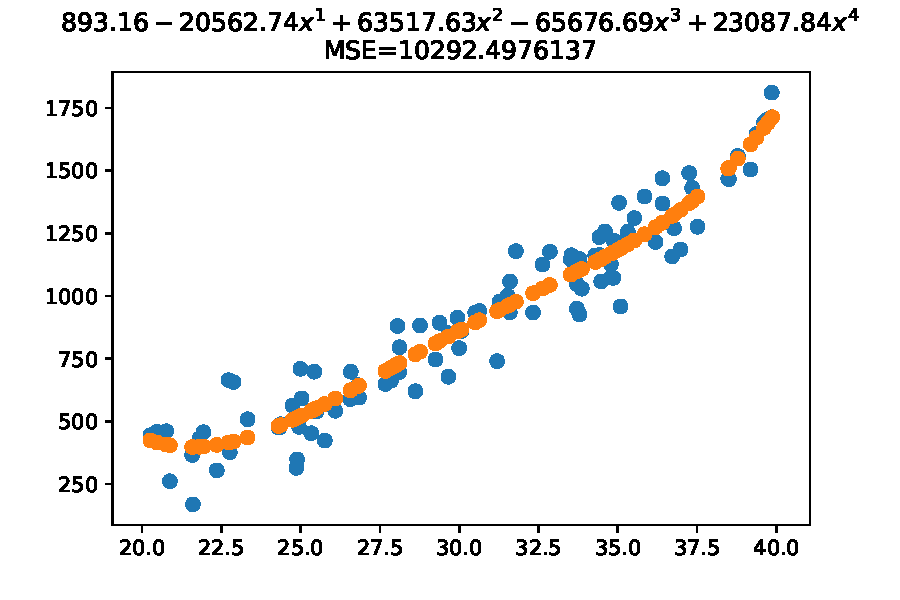
\includegraphics[width=\textwidth]{reg-2deg-with-noise-ridge0.pdf}
\end{frame}

\begin{frame}{Możliwe rozwiązanie (II)}
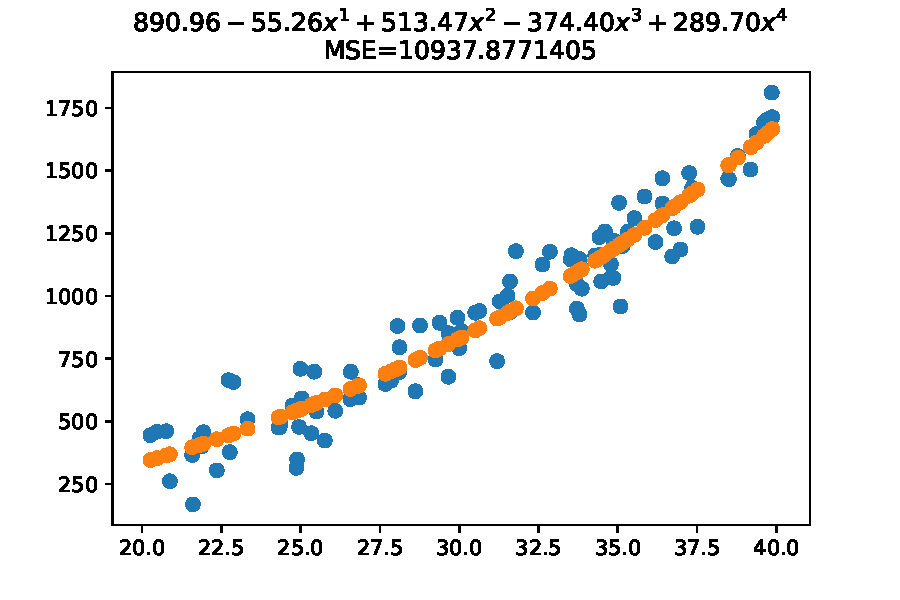
\includegraphics[width=\textwidth]{reg-2deg-with-noise-ridge0_001.pdf}
\end{frame}

\begin{frame}{Możliwe rozwiązanie (III)}
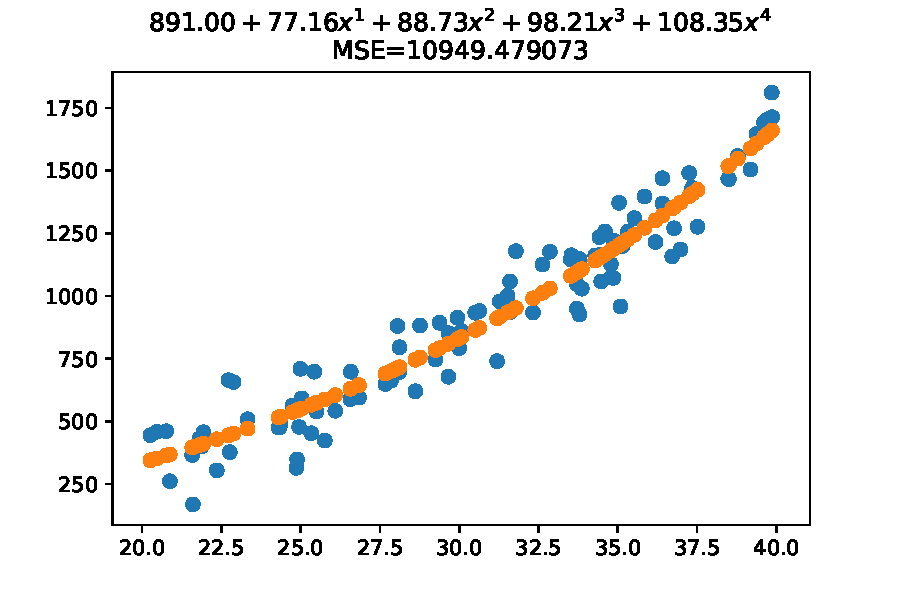
\includegraphics[width=\textwidth]{reg-2deg-with-noise-ridge1.pdf}
\end{frame}

\begin{frame}{Możliwe rozwiązanie (IV)}
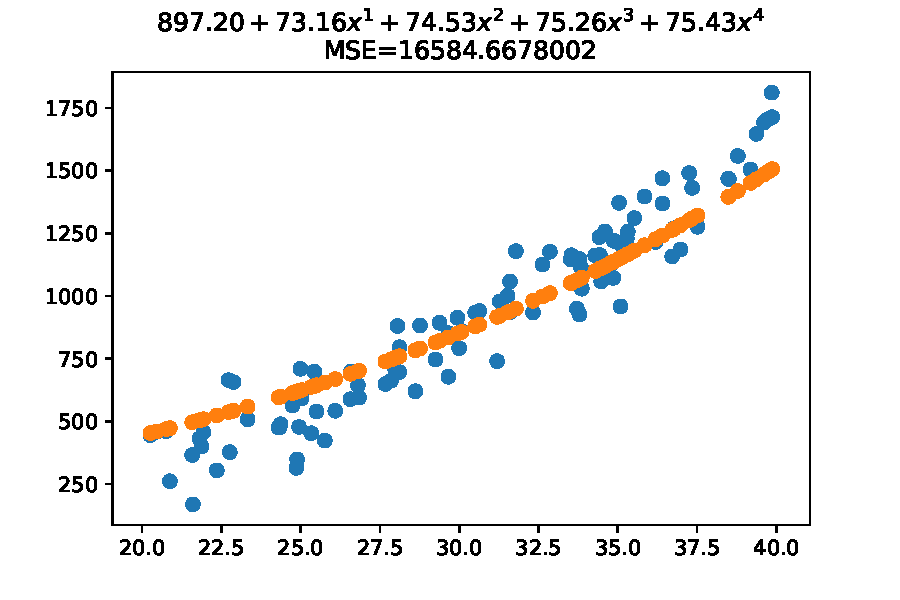
\includegraphics[width=\textwidth]{reg-2deg-with-noise-ridge100.pdf}
\end{frame}

\begin{frame}{Możliwe rozwiązanie (V)}
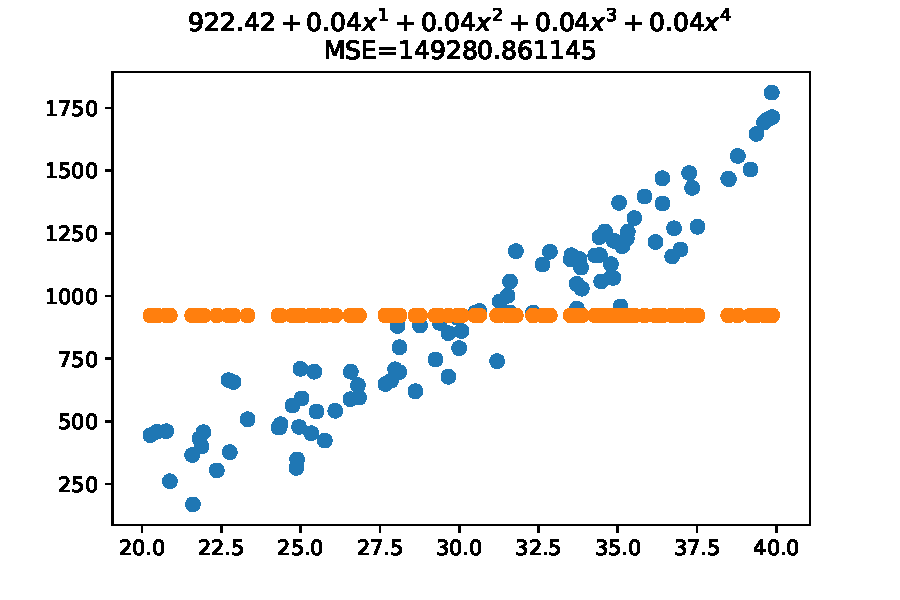
\includegraphics[width=\textwidth]{reg-2deg-with-noise-ridge1000000.pdf}
\end{frame}

\begin{frame}{Regularyzacja Ridge}
\[ J(\vec{w}) = MSE(\vec{w}) + \alpha \underbrace{\frac{1}{2}\sum_{\alert{i=1}}^n w_i^2}_{kara} \]
\end{frame}

\begin{frame}{Porównanie rozwiązań}
\centering
\begin{tabular}{rrrrrr}
$\alpha$ & $MSE_{tr}$  & kara  & całkowity koszt & $MSE_{walid}$ \\
\hline
$0$ & $10292$ & $4651895996$ & $10292$ & $9627$\\
$0.001$ & $10937$ & $245404$ & $11183$ & $8726$\\
$1$ & $10949$ & $17605$ & $28554$ & $8678$\\
$100$ & $16584$ & $11130$ & $1129591$ & $12312$\\
$1000000$ & $149280$ & $0$ & $152023$ & $138743$\\
\end{tabular}

\pause
\vfill
\alert{Ile współczynników miały rozważane wielomiany?}
\end{frame}

\begin{frame}{Możliwe rozwiązanie (I)}
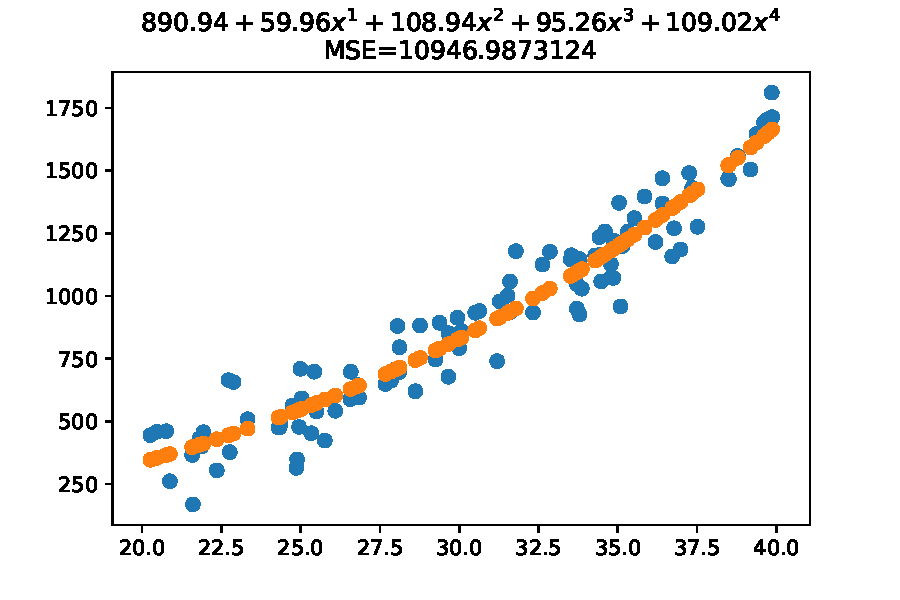
\includegraphics[width=\textwidth]{reg-3deg-with-noise-lasso0.pdf}
\end{frame}
\begin{frame}{Możliwe rozwiązanie (II)}
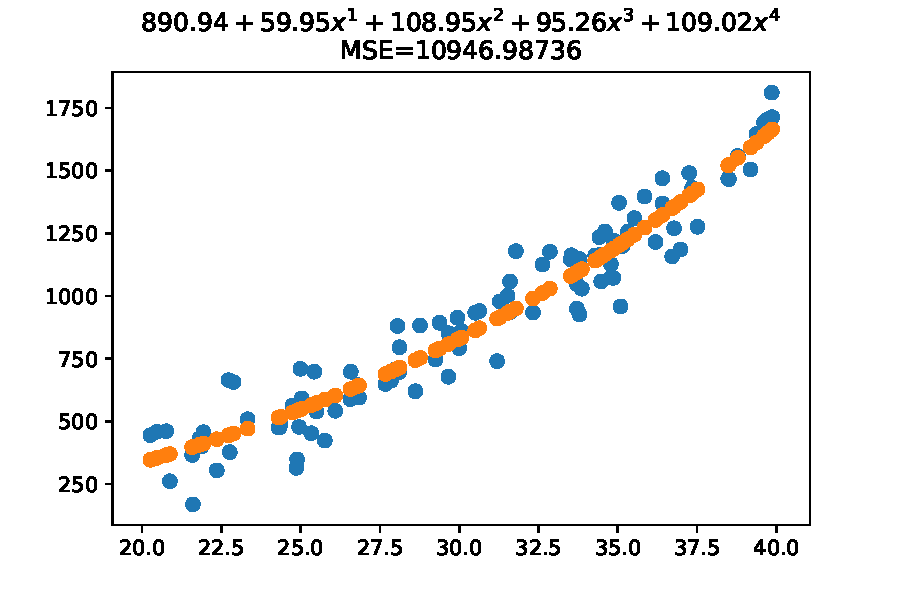
\includegraphics[width=\textwidth]{reg-3deg-with-noise-lasso0_001.pdf}
\end{frame}
\begin{frame}{Możliwe rozwiązanie (III)}
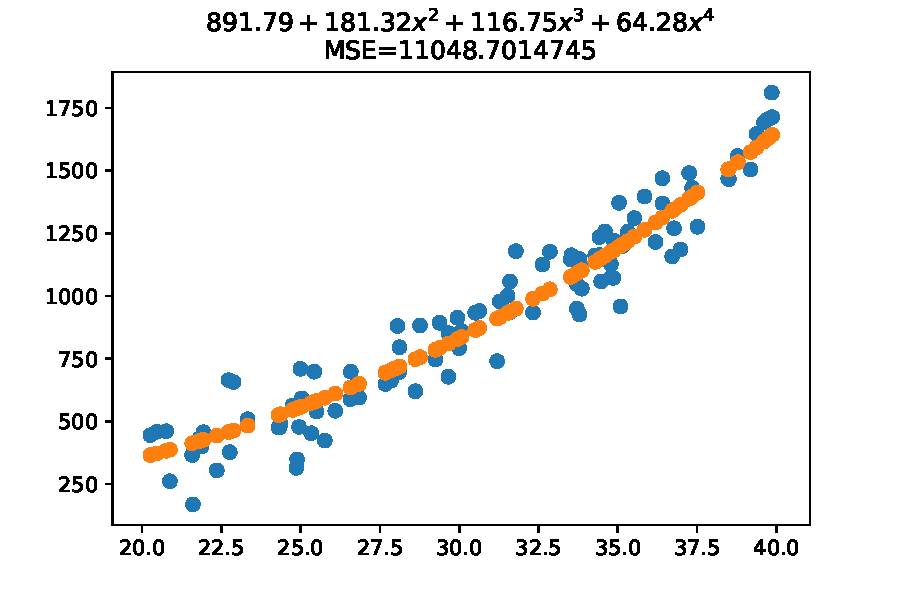
\includegraphics[width=\textwidth]{reg-3deg-with-noise-lasso10.pdf}
\end{frame}
\begin{frame}{Możliwe rozwiązanie (IV)}
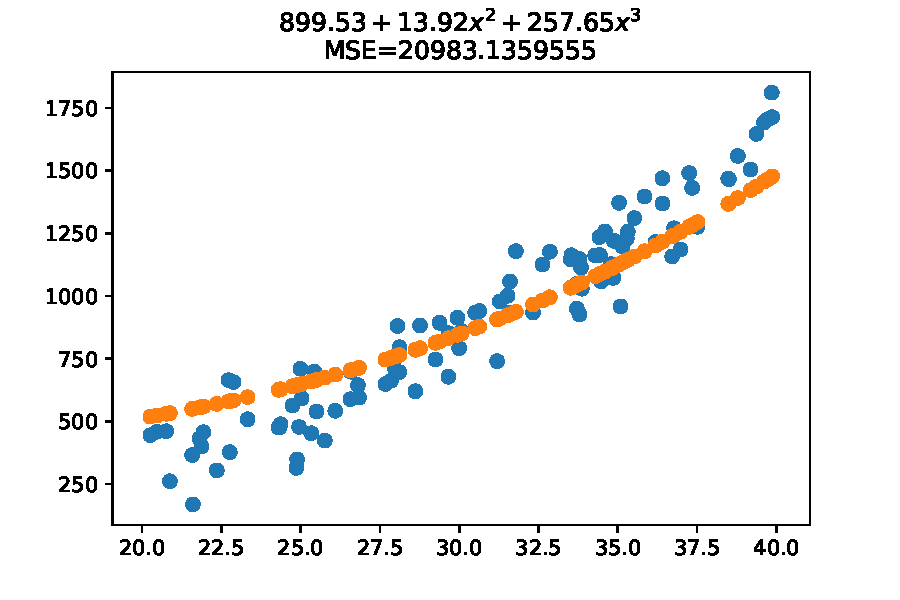
\includegraphics[width=\textwidth]{reg-3deg-with-noise-lasso100.pdf}
\end{frame}
\begin{frame}{Możliwe rozwiązanie (V)}
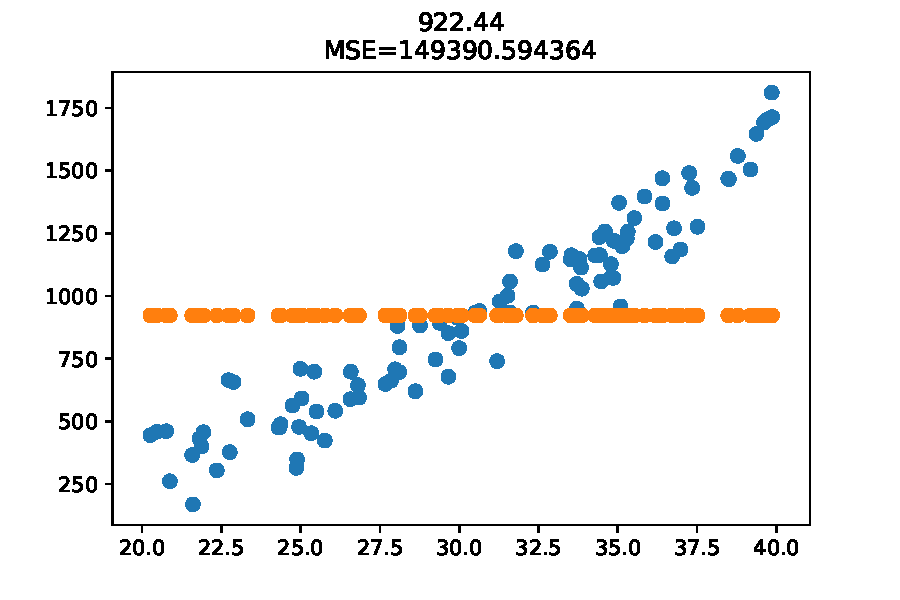
\includegraphics[width=\textwidth]{reg-3deg-with-noise-lasso1000000.pdf}
\end{frame}

\begin{frame}{Regularyzacja Lasso}
\[ J(\vec{w}) = MSE(\vec{w}) + \alpha \underbrace{\sum_{\alert{i=1}}^n \left|w_i\right|}_{kara} \]
\end{frame}

\begin{frame}{Porównanie rozwiązań}
\centering
\begin{tabular}{rrrrrrr}
$\alpha$ & \# wsp. & $MSE_{tr}$  & kara  & całkowity koszt & $MSE_{walid}$ \\
\hline
$0$ & $4$ & $10946$ & $18211$ & $10946$ & $8722$\\
$0.001$ & $4$ & $10946$ & $18211$ & $10965$ & $8721$\\
$10$ & $3$ & $11048$ & $25319$ & $264241$ & $8562$\\
$100$ & $2$ & $20983$ & $33287$ & $3349752$ & $16524$\\
$1000000$ & $0$ & $149390$ & $0$ & $149390$ & $138850$\\
\end{tabular}
\end{frame}

\begin{frame}{Dlaczego Lasso się tak zachowuje?}
Obliczmy karę w Ridge i w Lasso dla następujących przypadków:
\begin{enumerate}
\item \[ \vec{w}_1=\begin{bmatrix} 1 \\ 0.05 \end{bmatrix} \]
\pause
\item \[ \vec{w}_2=\vec{w}_1-\begin{bmatrix} 0.01 \\ 0 \end{bmatrix} \]
\pause
\item \[ \vec{w}_3=\vec{w}_1-\begin{bmatrix} 0 \\ 0.01 \end{bmatrix} \]
\end{enumerate}
\pause
\alert{Który przypadek jest lepszy dla regresji Ridge, a który dla Lasso?}
\end{frame}

\begin{frame}{Regularyzacja w GD: wczesne zatrzymanie}
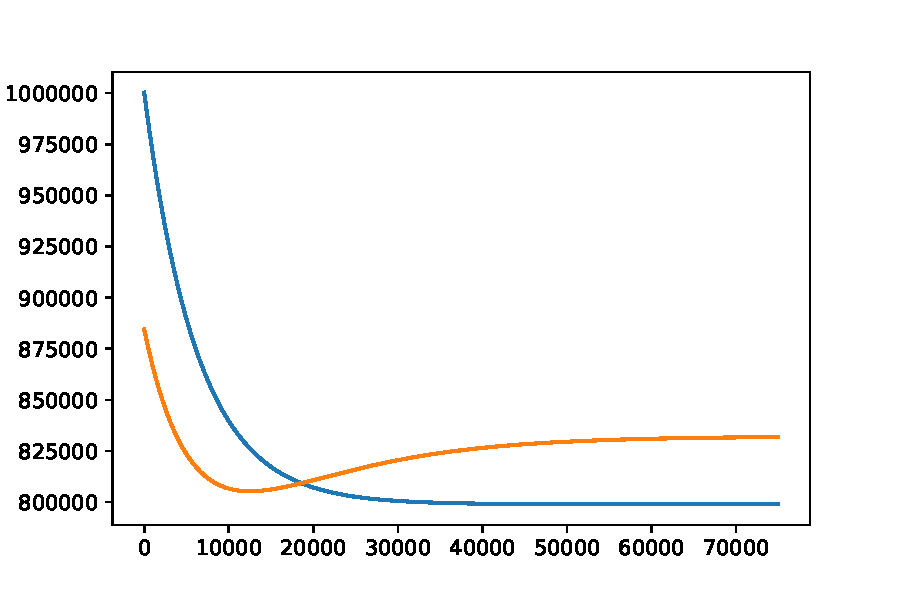
\includegraphics[width=\textwidth]{earlystopping.pdf}
\end{frame}

\end{document}